\documentclass[../manuscript.tex]{subfiles}

\section{Материалы и методы}
\subsection{Использованные данные}
\subsection{Алгоритмы предобработки данных}
Профессия вычислительного биолога подразумевает рутинную обработку больших гетерогенных данных, особенно что касается single-cell технологий. В связи с этим был реализован протокол предобработки данных секвенирования, основные шаги которого разобраны в данном разделе.
\begin{figure}[H]
	\centering
	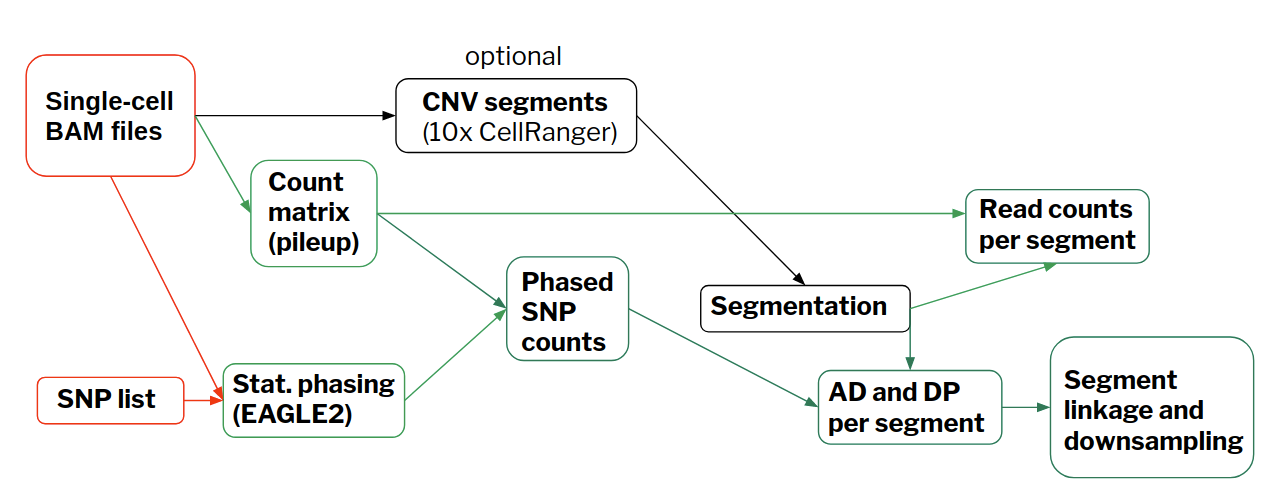
\includegraphics[keepaspectratio=true,scale=0.4]{images/preprocessing_pipeline.png}
	\caption{Граф протокола предобработки данных для алгоритма XClone. Красным обозначены входные данные, чёрным — опциональные шаги, зелёным — реализованные стадии.}
\end{figure}
\subsubsection{Извлечение данных из BAM-файлов}
\textbf{BAM} — \textit{binary SAM — binary sequence alignment/map format} — общепринятый формат сжатого хранения данных секвенирования. BAM-файл, полученный по протоколам 10x Genomics, занимает до нескольких терабайтов дискового пространства, потому эффективное извлечение информации из BAM-файлов это нетривиальная инженерная задача. Главные входные файлы XClone — матрицы прочтений. Таких матриц требуется три:
\begin{itemize}
	\item матрица $\mathrm{RD}$ всех прочтений достаточного качества;
	\item матрица $\mathrm{DP}$ всех прочтений, накрывающих хоть один ОНП в пределах сегментов; 
	\item матрица $\mathrm{AD}$ всех прочтений, накрывающих хоть альтернативный аллель ОНП в пределах сегментов.
\end{itemize}
Для получения матрицы $\mathrm{RD}$ из данных scRNA-seq был использован протокол \textbf{count} из \textbf{CellRanger}. Для всех остальных матриц во всех остальных случаях был использован \textbf{CellSNP}\footnote{https://github.com/single-cell-genetics/cellSNP}. 
\subsubsection{Статистическое фазирование гаплотипов} 
Гаплотипирование — определение того, от какого родителя унаследован каждый алллель в геноме — одна из ключевых задач генетики человека. Сложность её решения обусловлена контекстом, в котором она возникает в современных исследованиях, когда секвенируются порядка $2\cdot 10^{4}$ — $10^{6}$ позиций в геномах тысяч человек. Если прочтения короткие и не накрывают много позиций одновременно, то нужно секвенировать обоих родителей каждого участника эксперимента, что непрактично и не всегда возможно. Следовательно, нужно разрабатывать статистические методы гаплотипирования. Они основаны на наблюдении, что некоторые группы аллелей часто наследуются совместно. Это явление называется \textbf{неравновесной сцепленностью}. Если прогаплотипировано достаточное количество представителей популяции, то можно построить приближённые таблицы сцепленности и гаплотипировать новые образцы методом максимизации правдоподобия. 

На момент написания этого текста, стандартом статистического гаплотипирования считается алгоритм \textbf{EAGLE2}\cite{Eagle2}\footnote{https://data.broadinstitute.org/alkesgroup/Eagle/}. Этот алгоритм основан на скрытых марковских моделях и использует 32,470 образца из базы данных \textbf{Haplotype Reference Consortium}\cite{HaplotypeReferenceConsortium}.

Алгоритм EAGLE2 обладает существенным недостатком: его метки имеют только локальный смысл. В пределах окна в 20-50 килобаз любые два ОНП с одинаковой наследуются совместно, но при сдвиге окна смысл меток может спонтанно поменяться на противоположный, это так называемая \textbf{ошибка смены цепи}. Т.е. два ОНП с разных концов хромосомы, помеченые одной меткой, могут быть унаследованы от разных родителей. Из-за этого в матрицах прочтений размывается сигнал аллельного дисбаланса: чтобы сделать данные менее разреженными, прочтения соседних небольших сегментов суммируются, в том числе и аллель-специфичные. Ясно, что если среди двух соседних сегментов с одинаковой меткой один полностью унаследован от отца, а второй — от матери, то при сложении их аллель-специфичные сигналы скомпенсируют друг друга. Это, в свою очередь, приводит к неправильному предсказанию аллель-специфичных структурных вариаций и неправильной кластеризации клеток. Авторы EAGLE2 в переписке явно дали понять, что в общем случае  детектировать и исправлять такого рода ошибки их подход не позволяет. Но в контексте модели XClone удалось разработать статистический метод, показавший хорошие результаты при устранении ошибок переключения. Его подробное описание можно найти в одноимённом разделе.

\subsubsection{Подходы к сегментации генома}
Одной из основных задач XClone является предсказание \textbf{ASCNV} — аллель-специфических структурных вариаций генома. Это происходит в несколько этапов: (1) вначале определяются диапазоны, подозрительные на ASCNV, (2) затем их глубина покрытия сравнивается с эталонной для подсчёта RDR, (3) откуда получается оценка общего числа копий каждого конкретного диапазона, (4) которая затем уточняется при помощи сигналов аллельного дисбаланса. Наименее тривиальным из этих трёх шагов является первый: ни количество CNV, ни их границы заранее не известны. Тем не менее, на точность предсказания влияют ещё и технические факторы: \textbf{bin mappability} и \textbf{GC-contamination}.  

Bin mappability неформально стоит понимать как долю $k$-меров из заданного диапазона, которые однозначно выравниваются на этот же диапазон, где $k$ подчиняется Пуассоновской модели данных секвенирования. Если диапазон состоит из повторов одного короткого участка, то его mappability будет низкой, так как однозначно выравниваться будут только риды длиной больше половины от размера этого диапазона, вероятность которых будет мала. При заданной сегментации, эту величину можно с заданной точностью посчитать аналитически, но обычно для этого используют метод Монте-Карло.

Для отфильтровывания участков низкого качества используется \textbf{CellRanger DNA}, алгоритм\footnote{https://support.10xgenomics.com/single-cell-dna/software/pipelines/\\latest/algorithms/cnv\_calling} от 10X Genomics. Краткий обзор этого алгоритма представлен ниже:

Найденные участки накрывают некоторое подмножество референсного генома, которое затем подразделяется на сегменты размера 20-50 килобаз, в пределах которых вероятность ошибки смены цепи невелика, а потому сигнал аллельного дисбаланса статистически достоверный. Стоит отметить, что CellRanger DNA сам по себе является алгоритмом поиска CNV. Тем не менее, он сообщает, в том числе, и об участках без структурных вариантов. Благодаря этому можно гарантировать, что все участки генома, пригодные для надёжного определения ASCNV, войдут в итоговую сегментацию. 

\begin{figure}[H]
	\centering
	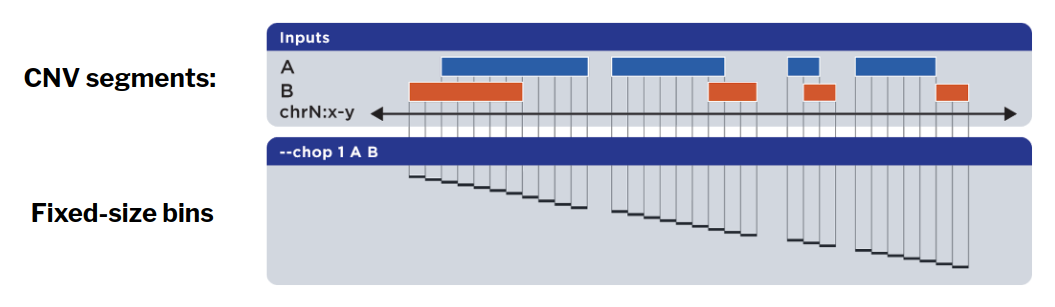
\includegraphics[keepaspectratio=true,scale=0.4]{images/segmentation.png}
	\caption{Иллюстрация алгоритма сегментирования генома. Длина индивидуальных сегментов задаётся заранее и выбирается из диапазона 20-50 килобаз. Подряд идущие фрагменты}
\end{figure}

В силу того, что структурные вариации обычно охватывают участки генома размеров хотя бы в несколько мегабаз, перед началом предсказания уместно аггрегировать подряд идущие сегменты в блоки фиксированного размера (обычно 1-5 мегабаз), чтобы получить менее шумные BAF и RDR. Тем не менее, наивно аггрегировать содержимое сегментов внутри блока — просуммировать числа прочтений — не получится, т.к. можно потерять аллель-специфический сигнал из-за ошибок смены цепи. В связи с этим был разработан алгоритм суммирования с коррекцией ошибок, который разобран в следующем разделе.

\subsubsection{Исправление ошибок смены цепи}
Поскольку одной из главных задач XClone является предсказание \textit{аллель-специфичных} структурных вариаций в геноме, матрицы $\mathrm{AD}$ и $\mathrm{DP}$ аллель-специфичных прочтений должны отражать биологию аллельного дисбаланса в клетках образца. Для этого нужно понимать, к какому гаплотипу принадлежит каждый ОНП. В разделе про статистическое гаплотипирование ОНП был сделан акцент на том, что существующие алгоритмы гарантируют только локальную корректность: при использовании алгоритма EAGLE2, следует ожидать, что при разбиении хромосомы на непересекающиеся окна длины 20-50 килобаз все гетерозиготные ОНП в пределах одного окна будут иметь одинаковый гаплотип, если это на самом деле так. Тем не менее, гаплотипы соседних сегментов с точки зрения алгоритма могут не совпадать даже тогда, когда на самом деле должны. К этому приводят так называемые \textbf{ошибки смены цепи} — спонтанная и неявная замена гаплотипических меток на противоположные внутри алгоритма. Классификацию ошибок переключения можно найти в статье \cite{Choi2018Plos}, цитата из которой приведена ниже:

\textit{"Phasing accuracy is typically measured by counting the number of \textbf{‘switches’} between known maternal and paternal haplotypes that should not occur if individual maternal and paternal chromosomal nucleotide sequence content has been accurately characterized. If an inconsistency is identified, then it is called a ‘switch error.’ These switch errors manifest themselves as induced and false recombination events in the inferred haplotypes compared with the true haplotypes. To identify \textbf{switch errors}, the phase of each site is compared with upstream neighboring phased sites. The switch error rate (SER) is defined as the number of switch errors divided by the number of opportunities for switch errors. Switch errors were further classified into three categories: \textbf{long}, \textbf{point}, and \textbf{undetermined}. A long switch appears as a large-scale pseudo recombination event; that is, there are no other switches in the local neighborhood around the long switch (e.g., no other switches within three consecutive heterozygous sites). On the contrary, a small-scale switch error appearing as two neighboring switch errors is considered as a point switch (e.g., two switches within three consecutive heterozygous sites, with the pair of switches counted as a point switch). The remaining switches are considered undetermined (e.g., only two sites phased in a small phasing block, so the switch error could not be classified into long or point)."}

Тем не менее, разбиение генома на фрагменты по 20-50 килобаз непрактично: в силу разреженности данных, в каждом таком сегменте может оказаться всего несколько ридов. Это даёт очень слабый и шумный сигнал аллельного дисбаланса. В связи с этим был разработан метод, одновременно решающий обе описанные проблем. На первом шаге алгоритма происходит разбиение генома на непересекающиеся сплошные сегменты длины $L$. Затем каждые $N$ подряд идущих сегментов объединяются в блок длины $NL$. В пределах блока переключения моделируются бернуллиевскими случайными величинами, по одной на каждый сегмент. Параметры этих распределений, в свою очередь, выводятся \textbf{ЕМ-алгоритмом}. После исправления ошибок, прочтения сегментов внутри блока суммируются, что даёт более стабильный сигнал. Эта идея была сформулирована в \cite{ChiselBiorxiv}, но технические детали были осознанно исключены авторами CHISEL из препринта. 

Прежде чем приступать к рассмотрению метода, сформулируем необходимые определения:

\begin{definition}[\textit{ЕМ-алгоритм}]$  $\\
EM-алгоритм (от английского \textit{"EM"} — \textit{"Expectation Maximization"}) — метод поиска оценок максимального правдоподобия (ОМП) или оценок апостериорного максимума (ОАП) параметров статистических моделей, содержащих скрытые переменные. 

\begin{algorithm}[H]
	\SetAlgoLined
	\KwResult{$\bm{\Theta}^{\ast},\ p(\bm{Z}\ |\ \bm{X}, \bm{\Theta}^{\ast})$}
	\text{$t = 0$}\;
	\text{$\bm{\Theta}^{(0)}$ инициализируется случайно}\;
	\While{$Q(\bm{\Theta}^{(t+1)}\ |\ \bm{\Theta}^{(t+1)}) - Q(\bm{\Theta}^{(t)}\ |\ \bm{\Theta}^{(t)}) > \eps$}{
		$\mathcal{L}(\bm{\Theta}^{(t)}; \bm{Z}, \bm{X}) := p(\bm{X}, \bm{Z}\ |\ \bm{\Theta}^{(t)})$\;
		$Q(\bm{\Theta}\ |\ \bm{\Theta}^{(t)}) := \mathbb{E}_{\bm{Z} | \bm{X}, \bm{\Theta}^{(t)}} \log \mathcal{L}(\bm{\Theta}; \bm{Z}, \bm{X})$ \tcp{E-шаг}
		$\bm{\Theta}^{(t+1)} := \arg\max\limits_{\bm{\Theta}} Q(\bm{\Theta}\ |\ \bm{\Theta}^{(t)})$ \tcp{M-шаг}
		$t = t + 1$
	}
	$\bm{\Theta}^{\ast} := \bm{\Theta}^{(t)}$
	\caption{ЕМ-алгоритм в общем виде}
\end{algorithm}

Здесь $\bm{Z}$ — дискретные скрытые переменные, $\bm{\Theta}$ — параметры статистической модели, $\bm{X}$ — выборка, $\eps > 0$. Каждая итерация алгоритма состоит из двух основных шагов:
\begin{enumerate}
	\item \textbf{Е-шаг}, на котором устраняется явная зависимость от скрытых переменных посредством взятия матожидания логарифма совместной функции правдоподобия по условному распределению $\bm{Z}\ |\ \bm{X}, \bm{\Theta}^{(t)}$;
	\item \textbf{M-шаг}, на котором параметры нового апостериорного распределения $\bm{\Theta}^{(t+1)}$ выбираются таким образом, чтобы максимизировать $ Q(\bm{\Theta}, \bm{\Theta}^{(t)}) $ — функцию правдоподобия "в среднем". 
\end{enumerate}
\end{definition}

С теоретическим обоснованием и формальным доказательством корректности EM-алгоритма можно ознакомиться в (\cite{MurphyProbabilisticML}, стр. 363-365). В контексте решаемой задачи $\bm{X}, \bm{Z}, \bm{\Theta}$ имеют следующий смысл:
\begin{itemize}
	\item $\bm{Z} = \{z_{1}, \ldots, z_{N}\}$ — независимые в совокупности индикаторы корректности гаплотипов сегментов
	\begin{gather*}
			\forall i: z_i \sim \mathrm{Bern}(p_i)\\
			\forall q \in \{0, 1\}^{N}: p(\bm{Z} = q\ |\ p_1, \ldots, p_n) = \prod_{i=1}^{N} p(z_i = q_i\ |\ p_i) = \prod_{i=1}^{N} p_i^{q_i} ( 1 - p_i)^{1-q_i}
	\end{gather*}
	Если $z_i = 1$, то будем говорить, что сегмент $i$ имеет корректный гаплотип, иначе — инвертированный. Эти обозначения имеют смысл только в пределах одного блока, в соседних блоках метки могут иметь противоположный смысл. Из этого наблюдения становится ясно, что алгоритм не решает проблему переключения полностью, но уменьшает число ошибок за счёт аггрегации сегментов в блоки.
	\item Обозначим через $M$ число клеток образца, тогда $\bm{X} = (\bm{X}_{1}, \ldots, \bm{X}_{M}),\ X_{c} := (\bm{a}_c, \bm{b}_c)$ —  вектора прочтений для каждой из клеток, по компоненте на сегмент.  $\bm{a}_c = (a_{c, 1}, \ldots, a_{c, N})$ — число прочтений аллеля А (альтернативный аллель), $\bm{b}_c =  (b_{c, 1}, \ldots, b_{c, N})$ — аллеля Б (референсный аллель).
	\item $\forall c \in \overline{1, M}: \bm{r}_c := \bm{a}_{c} + \bm{b}_{c}$ — вектора прочтений обоих аллелей вместе.
	\item $\bm{\Theta} = (\theta_1, \ldots, \theta_M; p_1, \ldots, p_N)$, где $\theta_c$ — пропорция ридов гаплотипа 1 в блоке в клетке $c$. Алгоритм предполагает, что пропорция гаплотипа 1 одинакова во всех сегментах внутри блока с точностью до переключения.
\end{itemize}
	
В этих обозначениях можно сформулировать и доказать следующее утверждение:
\begin{claim}
	Правила пересчёта параметров апостериорного распределения на М-шаге ЕМ-алгоритма имеют вид:
	\begin{equation}
		\begin{aligned}
			p_{i}^{(t+1)} &= \dfrac{ p_{i}^{(t)} \prod_{c=1}^{M} (\theta_{c}^{(t)})^{a_{c, i}} (1 - \theta_{c}^{(t)})^{b_{c, i}}}{p_{i}^{(t)} \prod_{c=1}^{M} (\theta_{c}^{(t)})^{a_{c, i}} (1 - \theta_{c}^{(t)})^{b_{c, i}} + (1 - p_{i}^{(t)}) \prod_{c=1}^{M} (\theta_{c}^{(t)})^{b_{c, i}} (1 - \theta_{c}^{(t)})^{a_{c, i}}}\\
			\theta_c^{(t+1)} &= \frac{\sum_{i=1}^{N}a_{i,c} \gamma^{(t)}_{i,1} + b_{i,c} \gamma^{(t)}_{i,0}}{\sum_{i=1}^{N} r_{i,c}}
		\end{aligned}
		\label{em_update_rules}
	\end{equation}
	где $\forall j \in \{0, 1\}: \gamma^{(t)}_{i,j} := P(z_i = j\ |\ \bm{X}, \bm{\Theta}^{(t)})$.
\end{claim}
\begin{proof}
  Вектора прочтений в клетках независимы в совокупности, потому: 
	\begin{gather*}
			P(\bm{X}\ |\ \bm{Z}, \bm{\Theta}) = \prod_{c=1}^{M} p(\bm{X}_c\ |\ \bm{Z}, \bm{\Theta}) = \prod_{c=1}^{N} \theta_{c}^{\widehat{a}_c(\bm{Z})}(1 - \theta_{c})^{\widehat{b}_c(\bm{Z})}
	\end{gather*}
	Где 
	\begin{gather*}
	\begin{cases}
		\widehat{a}_c(\bm{Z}) := \sum_{i=1}^{N} \left[z_i a_{c, i} + (1 - z_i) b_{c, i} \right],\\
		\widehat{b}_c(\bm{Z}) := \sum_{i=1}^{N} \left[(1 - z_i) a_{c, i} + z_i b_{c, i} \right],\\
		c \in \overline{1, M}
	\end{cases}
	\end{gather*}
	Тогда функция правдоподобия и её логарифм принимают вид
	\begin{align*}
			&\mathcal{L}(\bm{\Theta}; \bm{X}, \bm{Z}) = p(\bm{X}, \bm{Z} \ |\ \bm{\Theta}) = p(\bm{X}\ |\ \bm{Z}, \bm{\Theta}) p(\bm{Z}\ |\ \bm{\Theta})\\
			&l(\bm{\Theta}; \bm{X}, \bm{Z}) = \log \mathcal{L}(\bm{\Theta}; \bm{X}, \bm{Z}) =\\
			&= \log \prod_{\bm{q} \in \{0, 1\}^{N}} \left(\prod_{c=1}^{M} \theta_{c}^{\widehat{a}_c(\bm{q})}(1-\theta_{c})^{\widehat{b}_c(\bm{q})} \prod_{i=1}^{N} p_i^{q_i}(1-p_i)^{1-q_i}\right)^{\mathbb{I}\{\bm{Z} = \bm{q}\}} =\\
			&=\sum_{\bm{q} \in \{0, 1\}^{N}} \mathbb{I}\{\bm{Z} = \bm{q}\} \left( \sum_{c=1}^{M}\sum_{i=1}^{N} \widehat{a}_{c,i}(\bm{q}) \log \theta_{c} + \widehat{b}_{c,i}(\bm{q}) \log (1-\theta_{c})\right) +\\
			&+ \sum_{\bm{q} \in \{0, 1\}^{N}} \mathbb{I}\{\bm{Z} = \bm{q}\} \left(\sum_{i=1}^{N} q_{i} \log p_{i} + (1 - q_{i}) \log (1 - p_{i}) \right)
	\end{align*}
	Изменением порядка суммирования можно показать, что каждая из этих двух сумм распадается на $N$ сумм поменьше, по одной на каждую из скрытых переменных. В следствие этого и того, что компоненты случайного вектора $ \bm{Z} $ независимы в совокупности, шаги EM-алгоритма имеют вид:\\
	\noindent \textbf{E-шаг:}
	\begin{align*}
		&p(\bm{Z}\ |\ \bm{X}, \bm{\Theta}^{(t)})\ \propto\ p(\bm{X}\ |\ \bm{Z}, \bm{\Theta}^{(t)}) p(\bm{Z}\ |\ \bm{\Theta}^{(t)}) \implies\\
		&\implies \E_{\bm{Z}|\bm{X}, \bm{\Theta}^{(t)}} l(\bm{\Theta}; \bm{Z}, \bm{X}) = \sum_{i=1}^{N} \E_{\bm{z}_i|\bm{X}_i, \bm{\Theta}^{(t)}} \log \mathcal{L}(\bm{\Theta}; \bm{z}_i, \bm{X}_i) =\\
		&= \sum_{i=1}^{N} \sum_{q_i = 0}^{1} p(\bm{z}_i = q_i\ |\ \bm{X}_i, \bm{\Theta}^{(t)}) \left(
		\begin{aligned}
			&\sum_{c=1}^{M} \left[ \widehat{a}_{c,i}(q_i) \log \theta_{c} + \widehat{b}_{c,i}(q_i) \log (1 - \theta_{c}) \right] +\\
			&+ \log p(\bm{z}_i = q_i\ |\ \bm{\Theta})
		\end{aligned} \right) =\\
		&= \sum_{i=1}^{N} \left[ 
		\begin{aligned}
			&\gamma_{i,1}^{(t)} \left( \sum_{c=1}^{M} \left[a_{c,i} \log \theta_c + b_{c,i} \log(1-\theta_c) \right] + \log p_i \right) +\\ 
			&+ \gamma_{i,0}^{(t)} \left( \sum_{c=1}^{M} \left[b_{c,i} \log \theta_c + a_{c,i} \log(1-\theta_c) \right] + \log (1 - p_i) \right) 
		\end{aligned}
		\right] = Q(\bm{\Theta}\ |\ \bm{\Theta}^{(t)})
	\end{align*}
	
	\noindent \textbf{M-шаг:}
	\begin{gather*}
		p_{i}^{(t+1)} = \arg\max_{p_{i}} Q(\bm{\Theta}\ |\ \bm{\Theta}^{(t)}) \iff \frac{\gamma_{i, 1}^{(t)}}{p_{i}^{(t+1)}} - \frac{\gamma_{i, 0}^{(t)}}{1 - p_{i}^{(t+1)}} = 0 \iff p_{i}^{(t+1)} = \gamma_{i, 1}^{(t)}\\
		\begin{aligned}
			\theta_{c}^{(t+1)} = \arg\max_{\theta_c} Q(\bm{\Theta}\ |\ \bm{\Theta}^{(t)}) &\iff \frac{\sum_{i=1}^{N} \gamma_{i,1}^{(t)} a_{c, i} + \gamma_{i,0}^{(t)} b_{c, i}}{\theta_{c}^{(t+1)}} - \frac{\sum_{i=1}^{N} \gamma_{i,1}^{(t)} b_{c, i} + \gamma_{i,0}^{(t)} a_{c, i}}{1 - \theta_{c}^{(t+1)}} = 0\\
			&\iff \theta_c^{(t+1)} = \frac{\sum_{i=1}^{N} \gamma_{i,1}^{(t)} a_{c, i} + \gamma_{i,0}^{(t)} b_{c, i}}{\sum_{i=1}^{N} a_{c, i} +  b_{c, i}}
		\end{aligned}
	\end{gather*}
	Где необходимое условие локального экстремума является также достаточным в силу выпуклости функции $Q(\bm{\Theta}\ |\ \bm{\Theta}^{(t)})$ (\cite{MurphyProbabilisticML}, стр. 363-364).
\end{proof}
Стоит отметить, что на практике $p_{i}^{(t+1)}$ следует считать по эквивалетной, но уже численно устойчивой формуле:
\begin{gather*}
	p_{i}^{(t+1)} = \left(1 + \exp\left[\log(1 - p_{i}^{(t)}) - \log(p_{i}^{(t)}) + \sum_{c=1}^{M} \Delta_{c, i} (\log(\theta_{c}^{(t)}) - \log(1 - \theta_{c}^{(t)}))\right]\right)^{-1}
\end{gather*}
Где $\Delta_{c, i} := b_{c, i} - a_{c, i}$, а показатель экспоненты стоит искусственно приводить к диапазону $[-C; C]$ для некоторого $C > 0$ (авторами было выбрано $C = 100$). В противном случае $\prod_{c=1}^{M} (\theta_{c}^{(t)})^{a_{c, i}} (1 - \theta_{c}^{(t)})^{b_{c, i}}$ может представлять собой произведение тысяч или даже миллионов очень маленьких величин в больших степенях. Стандартной реализации чисел с плавающей запятой двойной точности недостаточно для хранения результатов промежуточных вычислений при использовании наивной формулы. 
\subsection{Первоначальная версия XClone: только ASE-модуль}
\subsubsection{Plate notation}
\subsubsection{Семплирование по Гиббсу}
\subsubsection{Предложенная модель, её недостатки}
\subsubsection{Unidentifiability problem, её решение в частном случае}
\subsection{Заключительная версия XClone: ASE- и RDR-модули}
\subsubsection{Вариационный байесовский вывод}
\subsubsection{Структура ASE-модуля}
\subsubsection{Структура RDR-модуля}
\subsubsection{Известные недостатки и планы по их исправлению}
